\documentclass{article}
\usepackage{graphicx}
\usepackage{subfigure}

\begin{document}

\section{Pneumatic Diagram}
\subsection{Inner Circuit}
\begin{figure}[h]
\centering
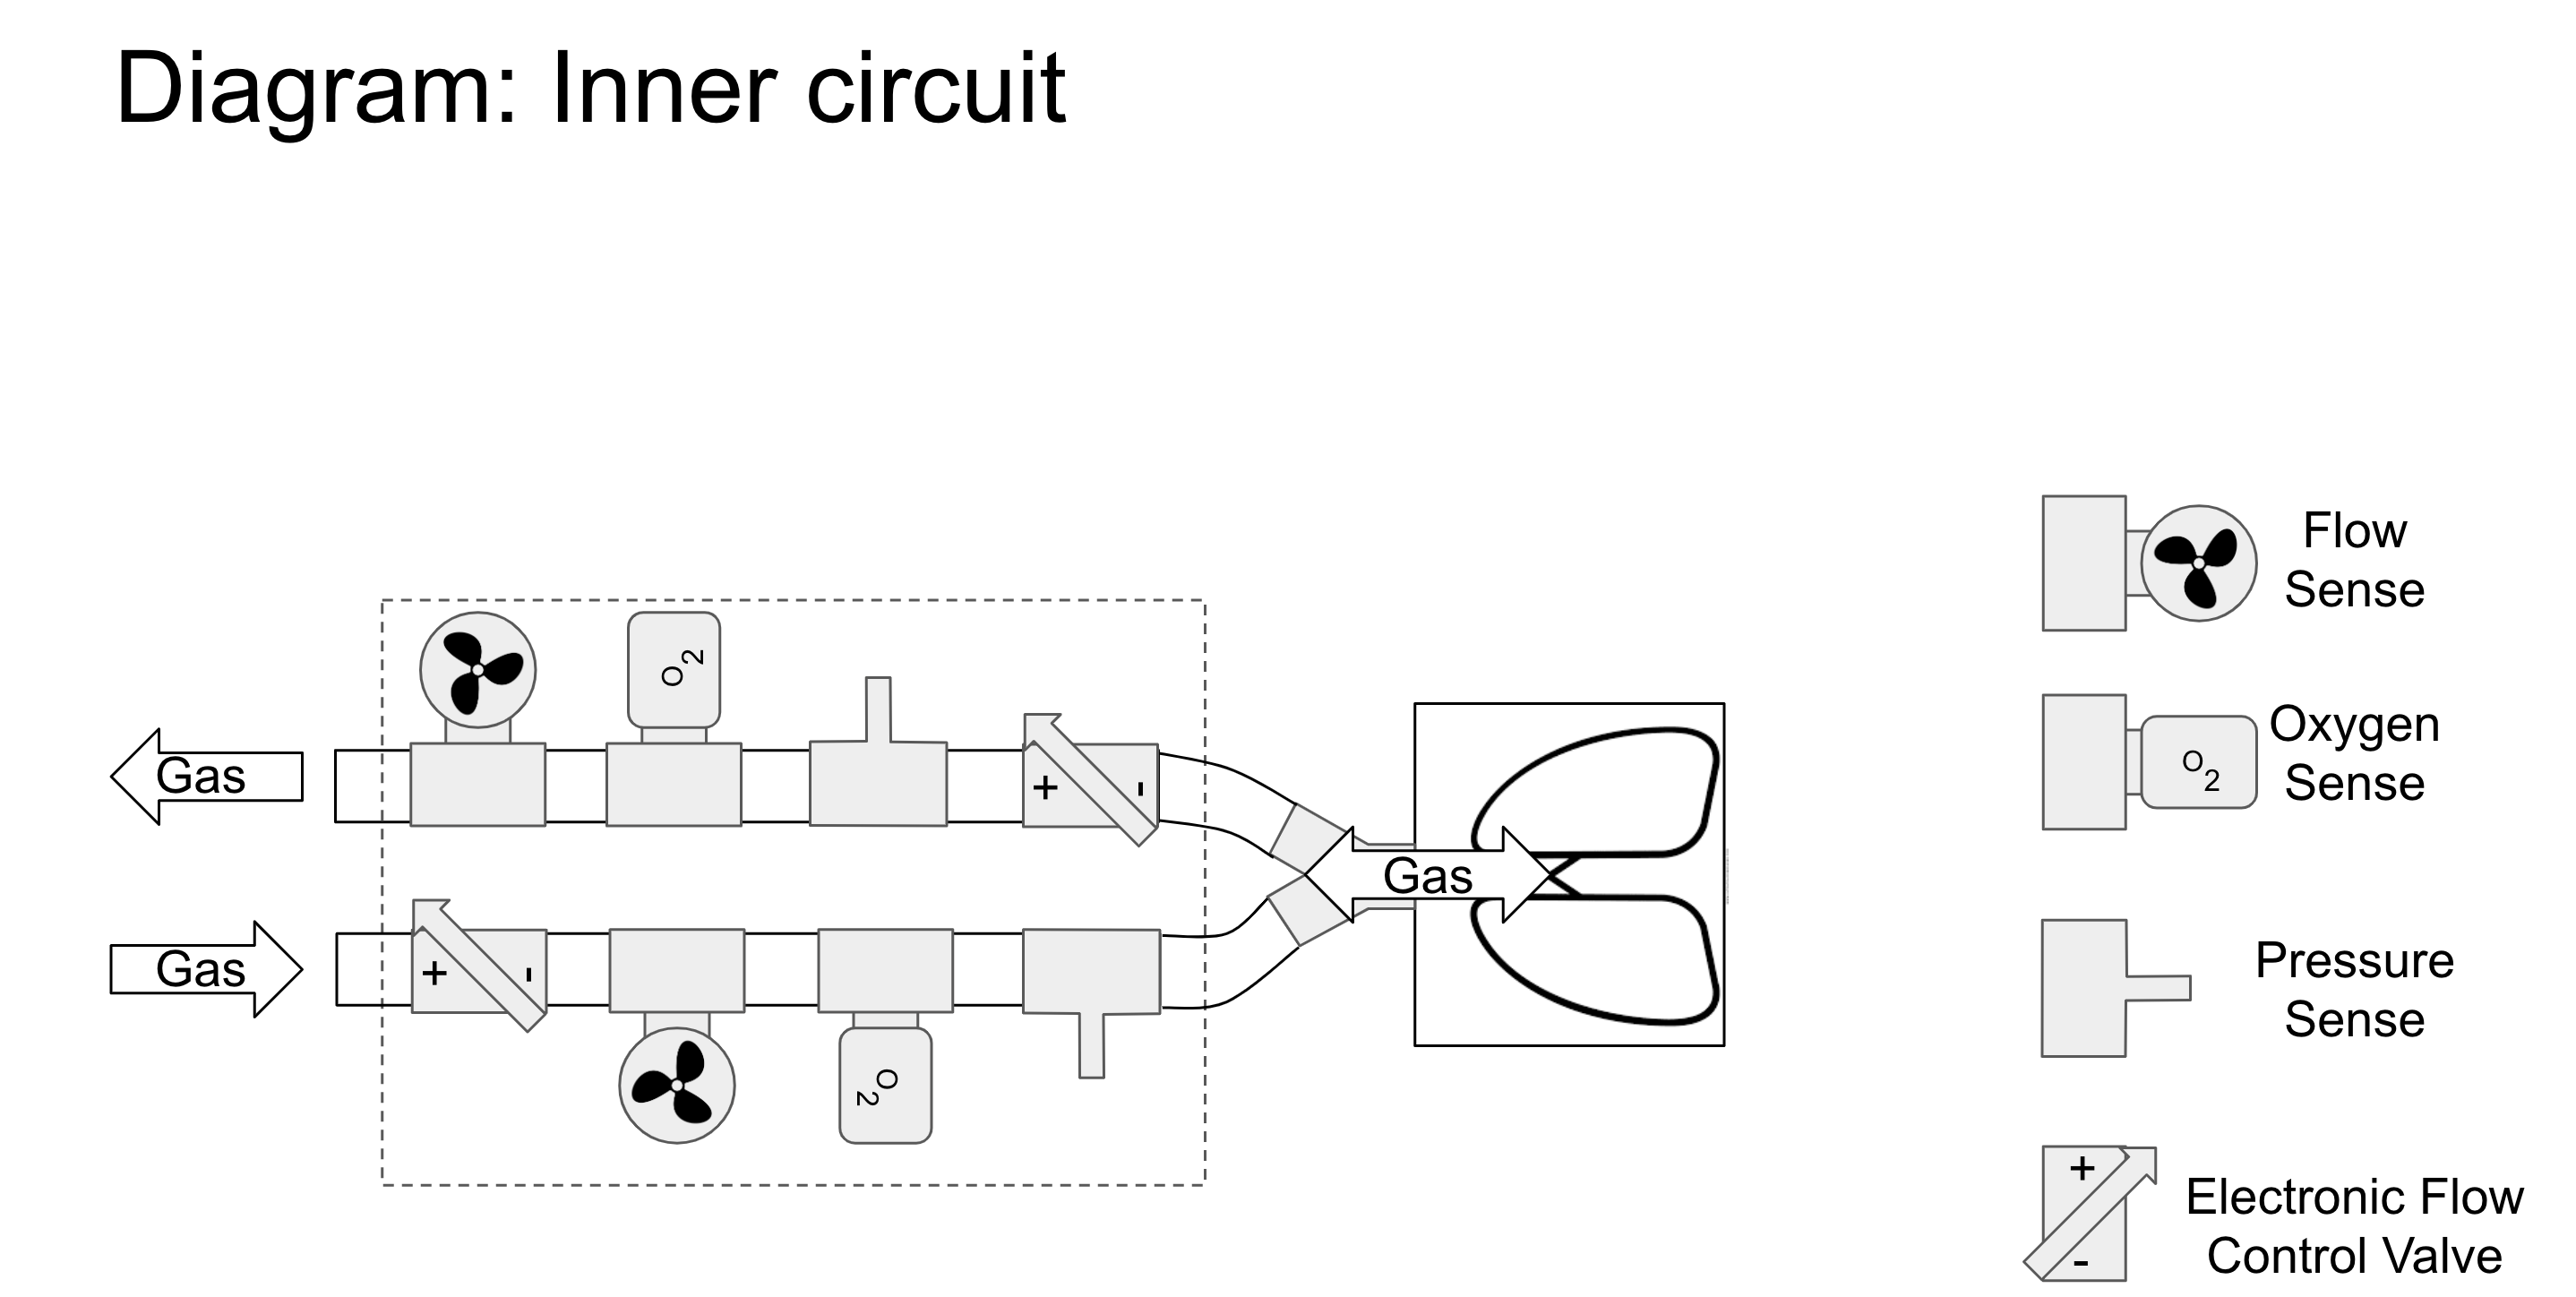
\includegraphics[scale=0.25]{pneumatic-diagram-inner.png}
\end{figure}

The two flow control valves will both be one-way. The lower tube is the inhalation tube and the upper tube is the exhalation tube.

\subsection{Outer Circuit}
\begin{figure}[h]
\centering
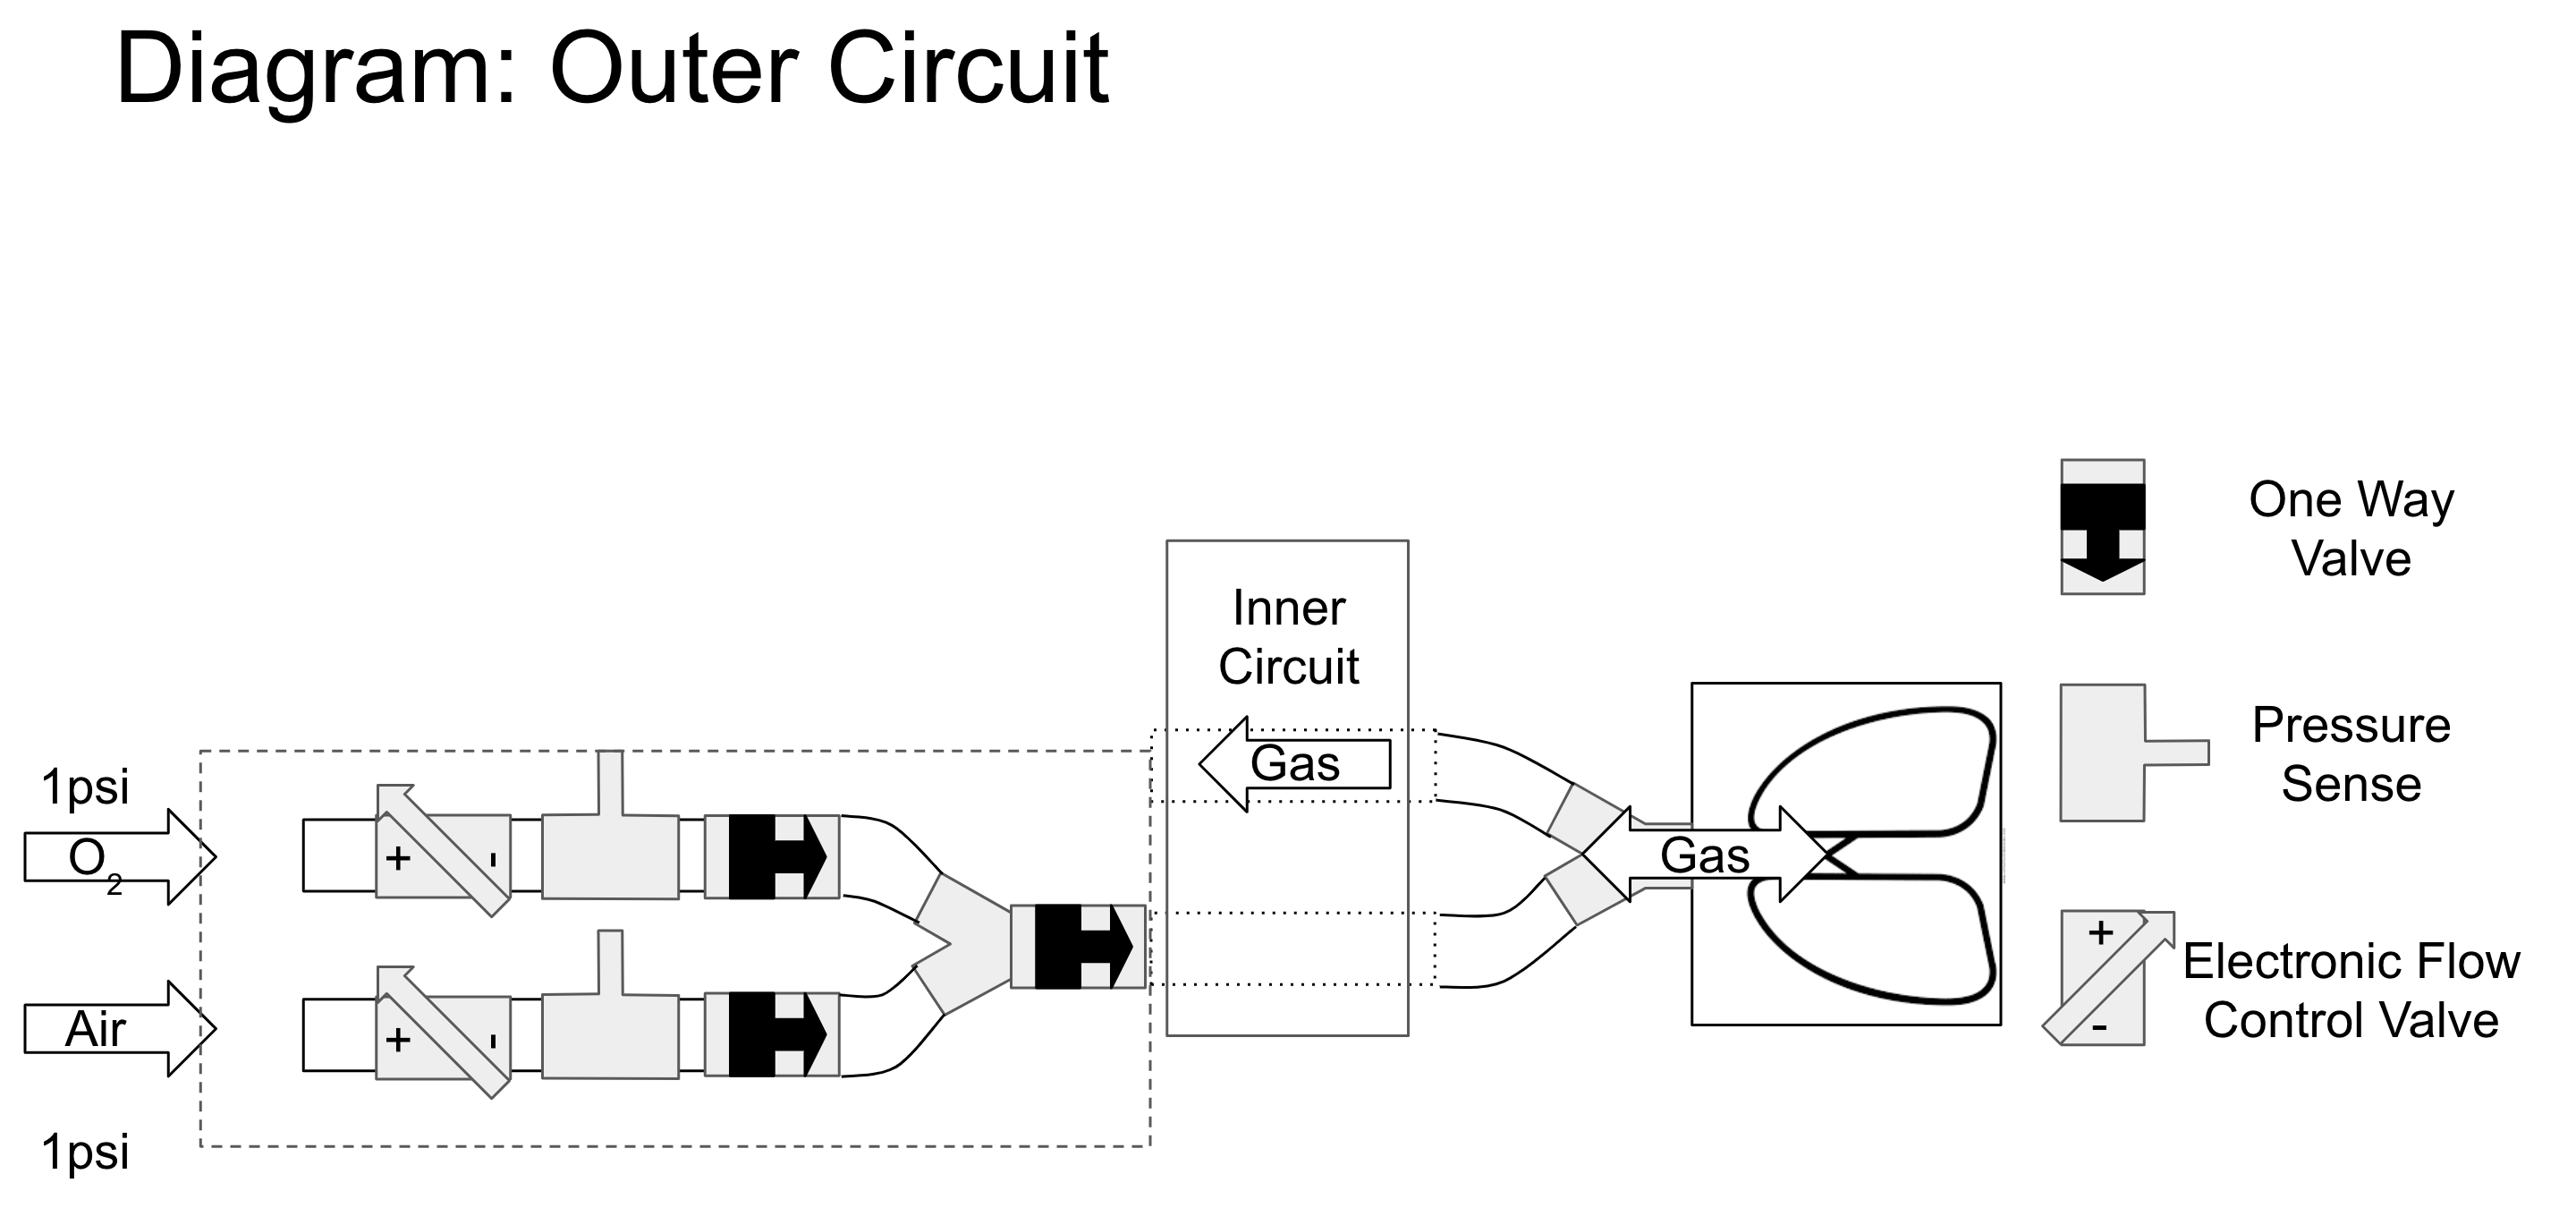
\includegraphics[scale=0.25]{pneumatic-diagram-outer.png}
\end{figure}

\newpage

\section{Inhalation}
\subsection{Control Circuit}
\begin{figure}[h]
\centering
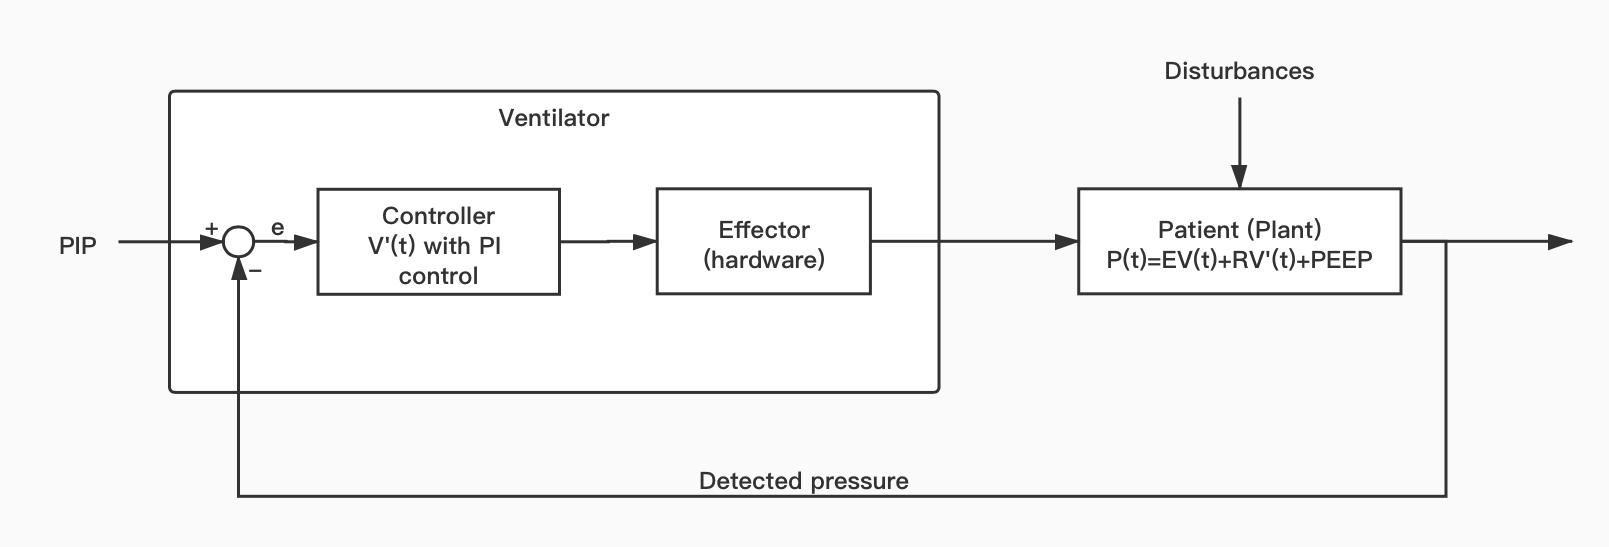
\includegraphics[scale=0.23]{control-circuit.jpg}
\end{figure}

The control circuit for inhalation. The input $PIP$ (Peak Inspiratory Pressure) is the expected level of pressure to reach. Error $e$ is the difference between actual pressure $P(t)$ measured by the sensor and $PIP$. $V(t)$ is the volume of air in patient's alveoli and $V'(t)$ would represent the flow speed of the injected gas. PI control is used in the circuit. The formula
$$P(t)=EV(t)+RV'(t)+PEEP$$
is the equation of motion, which shows a mathematical relation between the physical properties in the patient's lung. $E$ represents the elastance (inverse of the compliance) of the patient's lung and $R$ represents the airway resistance. $PEEP$ (Positive End Expiratory Pressure) is the remaining positive pressure in the patient's lung after exhalation. It is usually set as positive manually to prevent atelectasis. 

The formula for the controller is :
$$V'(t)=K_pe+K_i\int _0^tedt$$

\newpage

\subsection{Flow Diagram}
\begin{figure}[h]
\centering
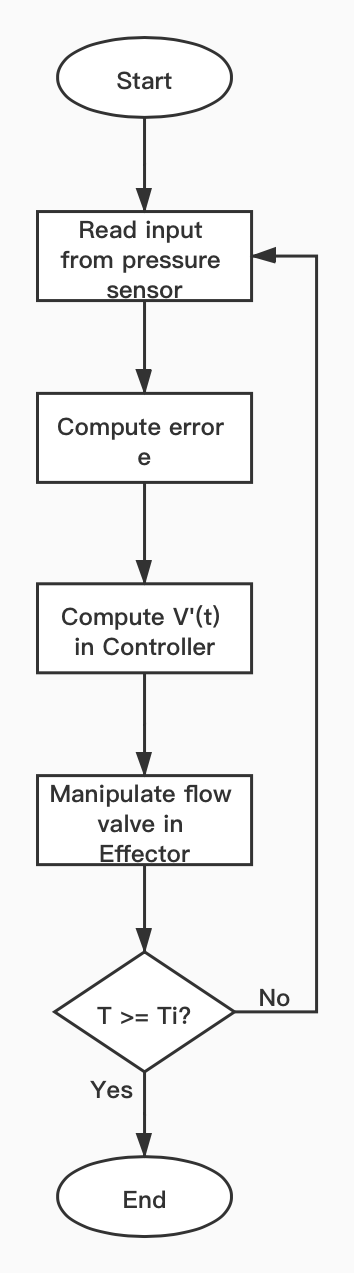
\includegraphics[scale=0.3]{flow-diagram.jpg}
\end{figure}

The flow diagram for a single inhalation. It can be triggered either by the machine or by patient. When the time $T$ has exceed the preset inspiratory time $Ti$, the inhalation would end and the exhalation would begin.

\newpage

\subsection{Transfer Function}
\begin{figure}[h]
\centering
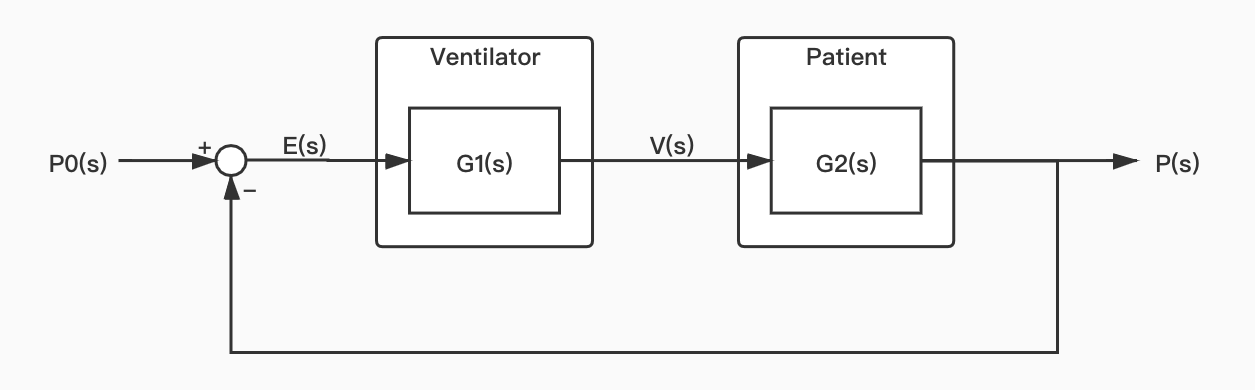
\includegraphics[scale=0.3]{block-diagram.jpg}
\end{figure}

$E(s), V(s)$, $P(s)$ is the Laplace transforms of the error $e(t)$, the volume $v(t)$ and the pressure $p(t)$. The input $P_{0}(s)$ is the Laplace transform of $p_{0}$, where $p_{0}$ is $PIP-PEEP$. $PEEP$ is subtracted from $PIP$ so that the zero initial condition of the system can be satisfied ($p(0)=0$). Notice that this doesn't change the property of the system, as when we pass the signal to the hardware, we can add the $PEEP$ back to the output $p(t)$ to transform from the relative pressure to the absolute pressure. Notice that  $G_1(s)$ is the transfer function of the ventilator and $G_2(s)$ is the transfer function of the patient.

For ventilator:
$$v'(t)=K_pe+K_i\int _0^tedt$$
Do Laplace transform on both sides:
$$sV(s)=K_pE(s)+\frac{K_i}{s}E(s)$$
$$G_1(s)=\frac{V(s)}{E(s)}=\frac{K_p}{s}+\frac{K_i}{s^2}$$

For patient:
$$p(t)=Ev(t)+Rv'(t)$$
Do Laplace transform on both sides:
$$P(s)=EV(s)+RsV(s)$$
$$G_2(s)=\frac{P(s)}{V(s)}=E+Rs$$
$$G(s)=\frac{P(s)}{E(s)}=G_1(s)\cdot G_2(s)=(\frac{K_p}{s}+\frac{K_i}{s^2})(E+Rs)$$
$$P(s)=G(s)\cdot E(s)=G(s)\cdot (P_0(s)-P(s))$$
$$\frac{P(s)}{P_0(s)}=\frac{G(s)}{1+G(s)}$$
Therefore, the transfer function of the system is:
$$\frac{P(s)}{P_0(s)}=\frac{G(s)}{1+G(s)}=\frac{K_pRs^2+(K_pE+K_iR)s+K_iE}{(K_pR+1)s^2+(K_pE+K_iR)s+K_iE}$$

\section{Exhalation}
The exhalation process is divided into two parts: 1. Let the gas in the patient's lung goes out naturally 2. Involve a PI control to maintain the pressure on a constant level ($PEEP$). 

For the first part, simply open the exhalation valve. However, instead of completely closing the inhalation valve, a basic flow is delivered by the inhalation tube to help the gas in the lung comes out.

For the second part, when the level of pressure has approached preset level ($PEEP$), a PI control will be triggered to maintain it. As for the PI control, all of the logic here is the same as in the inhalation process. In this case, the input for the control circuit will be $PEEP$ instead of $PIP$. The flow diagram of the program will be the same, and will ends when the preset time $T_e$ has been reached. The transfer function is also the same, with the input $P_0(s)$ being $0$ ($\Delta P=PEEP-PEEP=0$).

\section{Effector}
From the perspective of hardware, flow is manipulated by controlling the inhalation valve and exhalation valve. To get a positive flow, the inhalation valve will be opened accordingly and the exhalation valve will be closed. To get a negative flow, the exhalation valve will be opened accordingly and the inhalation valve will be closed. The effector will take in the calculated flow from the controller, and return PWM signals to the valves to control them.

\section{Inhalation-exhalation Cycle}
The length of the inhalation process and the exhalation process is determined by the preset parameters. The whole control program is conducted as infinitely repeating the inhalation-exhalation cycle. However, during the second half of the exhalation process, when the pressure has reached the $PEEP$ level (which basically means the patient has finished breathing out) and the next inhalation hasn't started, a patient-triggered breath is allowed. The patient will create a negative pressure in the lung when he/she want to start a spontaneous breath, and this can be detected by the pressure sensor. If an unusual large negative value of the difference between $PEEP$ and current pressure level has been detected during the time, the patient is trying to start a spontaneous breath. In this case, we will reset the Inhalation-exhalation cycle and start the inhalation process immediately.

\section{Intelligent Weaning Test}
The \textbf{rapid shallow breathing index} (RSBI) is an index that helps the doctors determine when to extubate the patient. RSBI is calculated by
$$RSBI=\frac{f}{V_T}$$, where $f$ is the respiratory frequency and $V_T$ is the tidal volume. At the current stage, we plan to add a function that can display RSBI to the doctors. For example, during every inhalation-exhalation cycle we can record the value of tidal volume, and every minute we can refresh the displayed RSBI by dividing total number of breaths in this minute by the average tidal volume.

\section{Compliance Tracking}
Compliance is an index that shows the physical property of the patient's lung. It is calculated by
$$\frac{1}{C}=\frac{plateau-peep}{V_T}$$, where $plateau$ is the plateau pressure during inhalation (also the peak inspiratory pressure in PCV), and $V_T$ is the tidal volume. Doctors may want to know the compliance of the patient to get an idea of his/her status. We plan to add a function that can display the patient lung's compliance to the doctor. We can record the the plateau pressure and tidal volume during every inhalation process and get the compliance of the patient's lung at that time.

\end{document}
